
\section{Modeling}

\subsection{Slum Mapping}

The primary purpose of the mapping models is twofold: to identify if there is some level of relationship between nighttime light values, population density, and the location of slums, and second to create a model that is able to provide data on slum locations to use later in the calibration of the household decision model. Due to restrictions on available computational power, this paper uses data only from surveyed slums in Kenya: as such, there is no need for any country level control variables. One key factor to remember is that since the following models only train on data from Kenya, any model interpretation will reveal only characteristics about Kenyan slums or slums in countries and cities that are very similar to Kenya.

\subsubsection{Model 1: Vanilla Logistic Regression}
We begin with a bare-bones logistic regression model. To discern the mixed effects of lights and population density, remember that we discretize the range of both of these values into five quantiles. We then interact these two new engineered categorical variables in the model. The initial logistic regression model is shown in Table 5.

% Table created by stargazer v.5.2.2 by Marek Hlavac, Harvard University. E-mail: hlavac at fas.harvard.edu
% Date and time: Sun, Apr 02, 2023 - 12:08:09 PM
\begin{table}[!htbp] \centering 
  \caption{Small extract from vanilla logit table} 
  \label{Vanilla Regression Table} 
\begin{tabular}{@{\extracolsep{5pt}}lc} 
\\[-1.8ex]\hline 
\hline \\[-1.8ex] 
 & \multicolumn{1}{c}{\textit{Dependent variable:}} \\ 
\cline{2-2} 
\\[-1.8ex] & slum \\ 
\hline \\[-1.8ex] 
  Light Bin 4 and Pop Density Bin 0 & 2.611$^{***}$ \\ 
  & (0.404) \\ 
  & \\ 
 Light Bin 0 and Pop Density Bin 4 & 1.430$^{***}$ \\ 
  & (0.398) \\ 
  & \\ 
 Light Bin 4 and Pop Density Bin 1 & $-$2.050$^{***}$ \\ 
  & (0.410) \\ 
  & \\
 Light Bin 4 and Pop Density Bin 4 & $-$2.085$^{***}$ \\ 
  & (0.409) \\ 
  & \\ 
\hline \\[-1.8ex] 
Observations & 31,810 \\ 
Log Likelihood & $-$20,911.600 \\ 
Akaike Inf. Crit. & 41,863.200 \\ 
\hline 
\hline \\[-1.8ex] 
\textit{Note:}  & \multicolumn{1}{r}{$^{*}$p$<$0.1; $^{**}$p$<$0.05; $^{***}$p$<$0.01} \\ 
\end{tabular} 
\end{table} 

These results bode well for the initial hypothesis that slums tend to appear in areas with low light level values, but also seems to indicate that in general, low light level values are a good indicator of slums regardless of population density, and the biggest factor that contributes towards areas not being considered as slums is the highest bin of light values. Results for population density are a bit more inconclusive in terms of determining a general trend. Ultimately, the biggest takeaway is that low light level values drive the biggest increase in the log odds of a specific geo-coordinate observation being considered a slum and the highest light level values are the biggest drivers of decreasing the log odds of a specific geo-coordinate observation being considered a slum.

Although there seems to be promising statistical significance results it is important to assess the predictive ability of this model as well. Logistic regression prediction often considers a prediction probability threshold of 0.5, this is, however, one hyperparameter than can be tuned and optimized for the sake of arriving at a better predictive model. 

%latex table generated in R 4.0.3 by xtable 1.8-4 package
% Tue Feb 07 21:15:33 2023
\begin{table}[ht]
\centering
\caption{Logit Model 1 Validation error metrics}
\begin{tabular}{llll}
  \hline \hline 
  Error Metric &  Slum Predictions &  Slum Observations  & Error Rate \\ 
  \hline
Total data set & 2696 & 10604 & 0.4048472 \\ 
Positive Slum Observations & 1525 & 4647 & 0.6718313\\
   \hline
\end{tabular}
\end{table}

After conducting a grid search through potential threshold values we see that we can drastically increase slum predictive accuracy while only sacrificing a little accuracy in the context of the entire data set. Finally, Figure 15 provides a spatial view of how the model seems to be performing using a prediction threshold of 0.4.

\begin{figure}
    \centering
    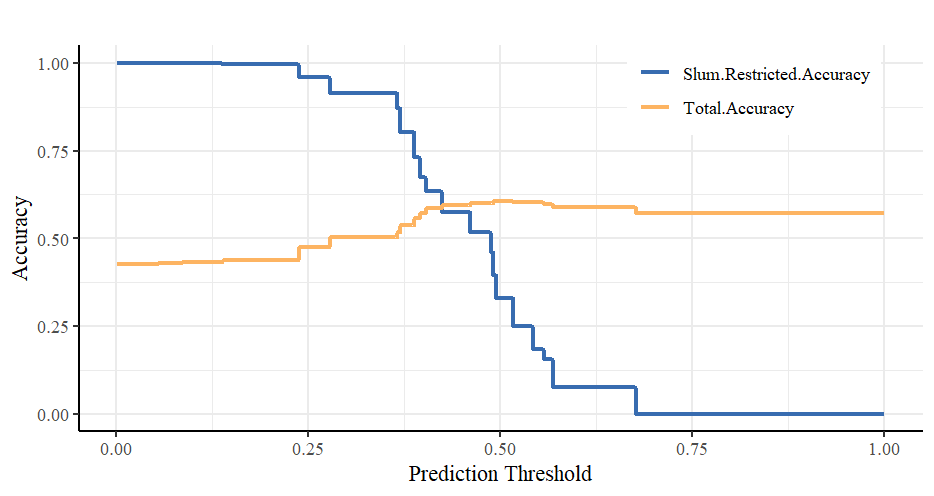
\includegraphics[scale = 0.8]{Graphics/Vanilla Slums and Total Dataset Accuracy Tradeoff.png}
    \caption{Vanilla Logit Slums and Total data set Accuracy Tradeoff}
    \label{fig:vanillaModelTradeoff}
\end{figure}

\begin{figure}
    \centering
    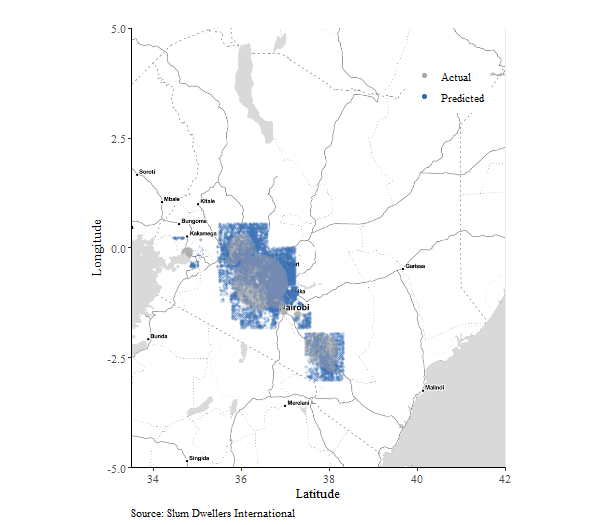
\includegraphics[scale = 0.7]{Graphics/Vanilla Predicted Spatial Distribution of Slums in Kenya.png}
    \caption{Vanilla Logit Model Predicted Spatial Distribution of Slums in Kenya}
    \label{fig:vanillaPredict}
\end{figure}

\subsubsection{Model 2: Logit with Increased Bins}

Having a data set with only five bins creates a lot of potential for categorizing values that are drastically different from each other into the as the same bin value. One way to address this issue is to increase the number of bins. 

\begin{figure}
    \centering
    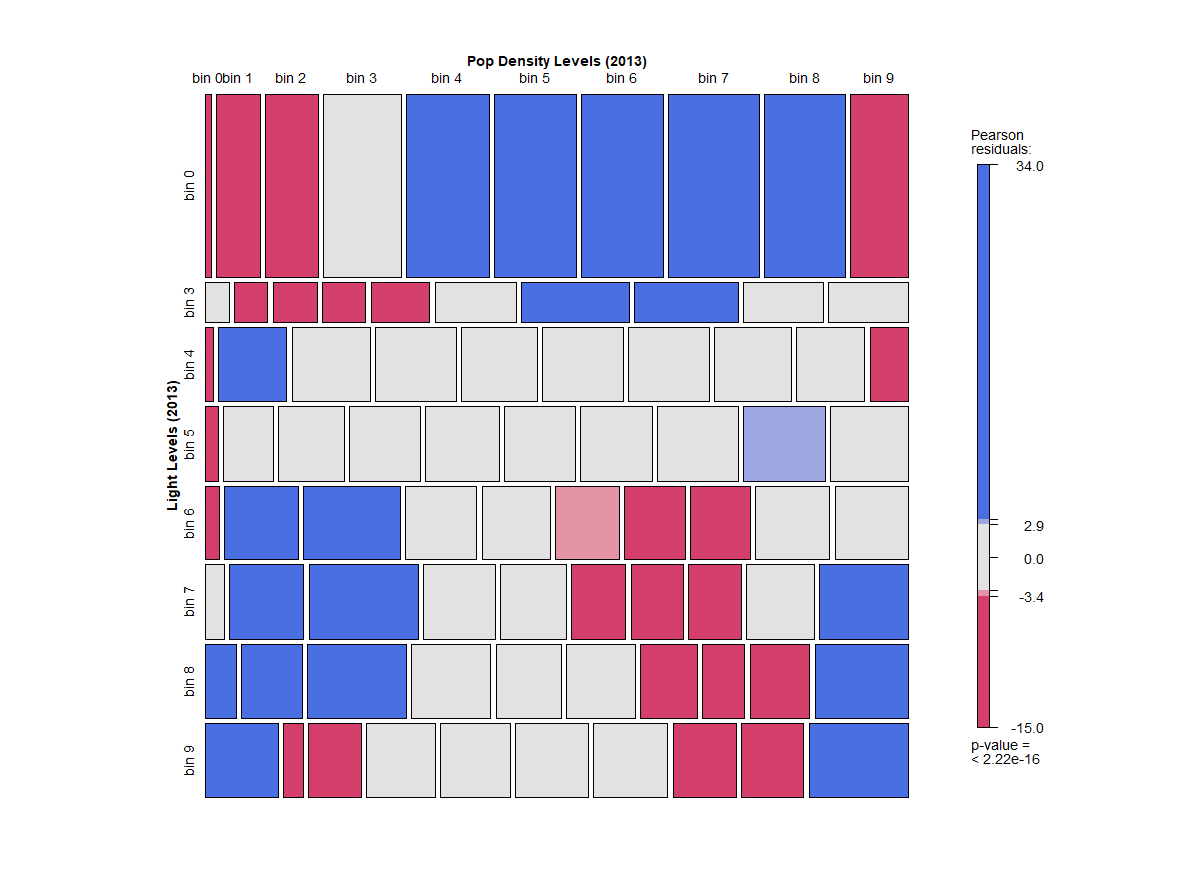
\includegraphics[scale = 0.225]{Graphics/Total Mosaic Bins.png}
    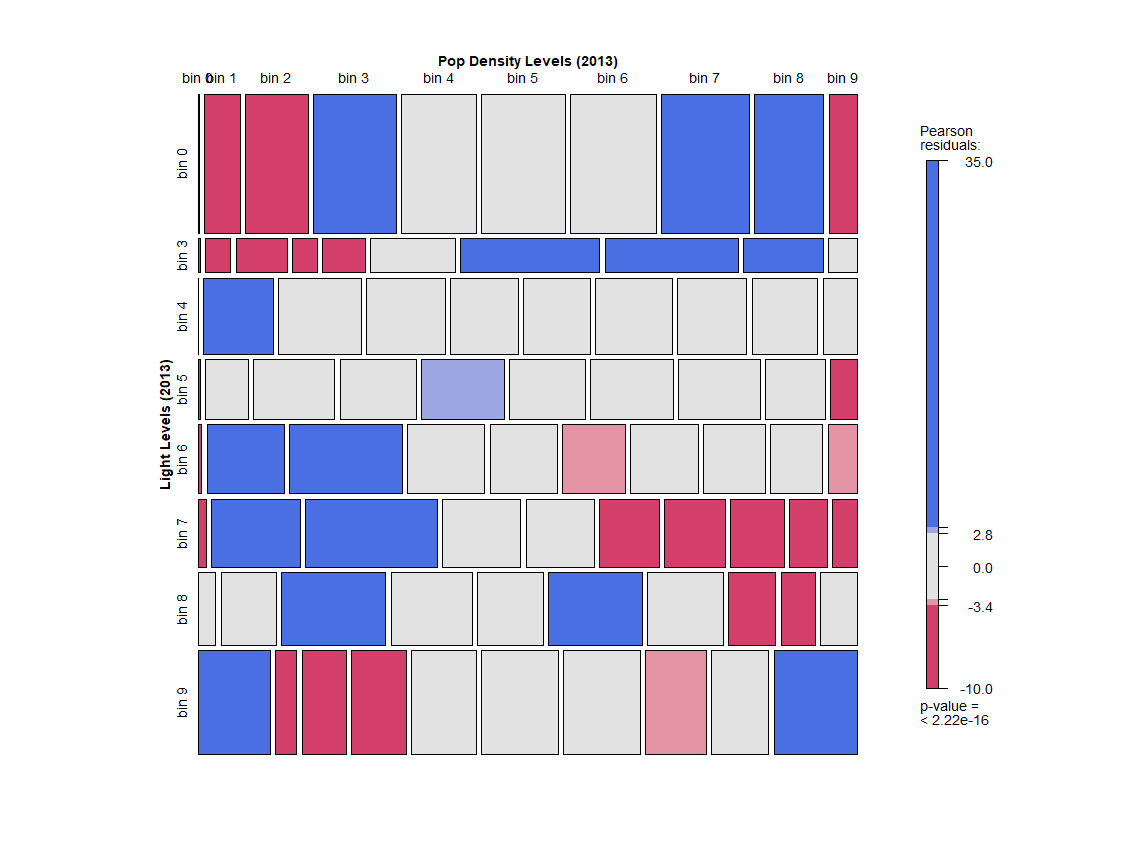
\includegraphics[scale = 0.23]{Graphics/Slum Mosaic Bins.png}
    \caption{Mosaic plot with 10 bins shows similar levels of heterogeneity in distribution of lights and population density}
    \label{fig:binsMosaic}
\end{figure}

Again, the mosaic plots indicate a similar story as with the data with just five bins. There is, however, additional nuance with the extreme high light and population density values.

% Table created by stargazer v.5.2.2 by Marek Hlavac, Harvard University. E-mail: hlavac at fas.harvard.edu
% Date and time: Sun, Apr 02, 2023 - 12:11:57 PM
\begin{table}[!htbp] \centering 
  \caption{Small extract of bins logit regression table} 
  \label{Bins Regression Table} 
\begin{tabular}{@{\extracolsep{5pt}}lc} 
\\[-1.8ex]\hline 
\hline \\[-1.8ex] 
 & \multicolumn{1}{c}{\textit{Dependent variable:}} \\ 
\cline{2-2} 
\\[-1.8ex] & slum \\ 
\hline \\[-1.8ex] 
Light Bin 0 and Pop Density Bin 8 & 1.632$^{***}$ \\ 
  & (0.400) \\ 
  & \\ 
 Light Bin 9 and Pop Density Bin 2 & $-$2.616$^{***}$ \\ 
  & (0.435) \\ 
  & \\ 
 Light Bin 4 and Pop Density Bin 9 & 1.864$^{**}$ \\ 
  & (0.842) \\ 
  & \\ 
 Light Bin 9 and Pop Density Bin 9 & $-$1.386$^{***}$ \\ 
  & (0.430) \\ 
  & \\ 
\hline \\[-1.8ex] 
Observations & 31,810 \\ 
Log Likelihood & $-$20,442.560 \\ 
Akaike Inf. Crit. & 41,045.130 \\ 
\hline 
\hline \\[-1.8ex] 
\textit{Note:}  & \multicolumn{1}{r}{$^{*}$p$<$0.1; $^{**}$p$<$0.05; $^{***}$p$<$0.01} \\ 
\end{tabular} 
\end{table} 


Once more, the regression results relate a remarkably similar story as with the logistic regression model with only five bins. As a whole, the predictive capabilities of this model seem to be a bit worse than that of the normal logistic regression with 5 bins with respect to general error metrics at a predictive threshold of 0.5. Again after conducting a gridsearch through potential threshold values, however, we see that we can drastically increase slum predictive accuracy while only sacrificing a little accuracy in the context of the entire data set a bit more than the previous regression model with only five bins. Finally, Figure 18 provides a spatial view of how the model seems to be performing using a prediction threshold of 0.4 and shows how it is able to mark one more slum area near Kakamega which the previous model was not able to do.

\begin{figure}
    \centering
    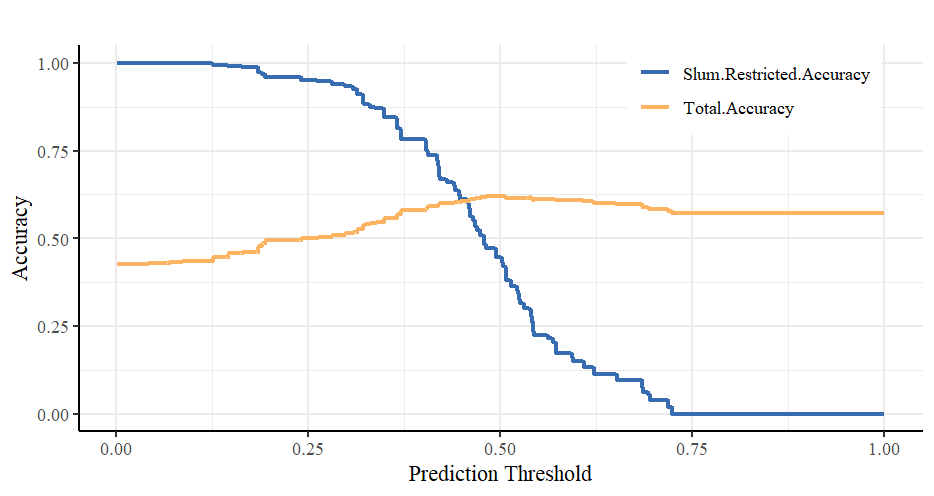
\includegraphics[scale = 0.8]{Graphics/Bins Slums and Total Dataset Accuracy Tradeoff.png}
    \caption{Bins Logit Model Slums and Total data set Accuracy Tradeoff}
    \label{fig:binsModelTradeoff}
\end{figure}



\begin{figure}
    \centering
    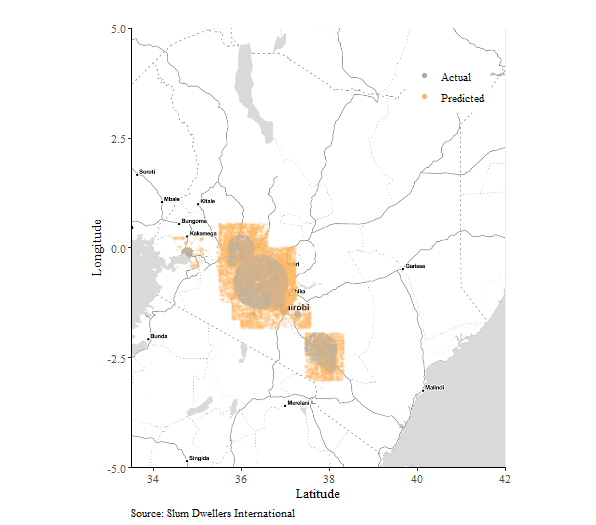
\includegraphics[scale = 0.6]{Graphics/Bins Predicted Spatial Distribution of Slums in Kenya.png}
    \caption{Bins Logit Model Predicted Spatial Distribution of Slums in Kenya}
    \label{fig:binsPredict}
\end{figure}

%latex table generated in R 4.0.3 by xtable 1.8-4 package
% Tue Feb 07 21:15:33 2023
\begin{table}[ht]
\centering
\caption{Logit Model 2 Validation error metrics}
\begin{tabular}{llll}
  \hline \hline
  Error Metric &  Slum Predictions &  Slum Observations  & Error Rate \\ 
  \hline
Total data set & 2759 & 10604 & 0.3904187 \\ 
Positive Slum Observations & 1651 & 4638 & 0.6474482\\
   \hline
\end{tabular}
\end{table}
\subsubsection{Model 3: Weighted Logit}



Within the current data set, the distribution of slums and no slum data points is relatively balanced. This property may not, however, extrapolate to other cities or data sets that undergo less pre-processing to consider only data from select cities and rural areas. Models trained on this data are drastically unbalanced and favor negative predictions resulting in models with exceptionally low overall accuracy but near a near 100\% false positive rate. As such, to better adapt to future applications of this research onto different data sets we also consider a weighted logistic regression that is biased towards slums. In the case of this initial model, we double weight slums relative to no-slum observations. The regression results are in Table 9 and indicate a similar story to the other models as well. Locations that have low light levels and high population density increase the likelihood of that location being a slum but more so high light level values decrease the likelihood of a location being a slum regardless of the population density level of that area.

%latex table generated in R 4.0.3 by xtable 1.8-4 package
% Tue Feb 07 21:15:33 2023
\begin{table}[ht]
\centering
\caption{Logit Model 3 Validation error metrics}
\begin{tabular}{llll}
  \hline \hline
  Error Metric &  Slum Predictions &  Slum Observations  & Error Rate \\ 
  \hline
Total data set & 9055 & 10604 & 0.3564527 \\ 
Positive Slum Observations & 2997 & 4657 & 0.35645265\\
   \hline
\end{tabular}
\end{table}

% Table created by stargazer v.5.2.2 by Marek Hlavac, Harvard University. E-mail: hlavac at fas.harvard.edu
% Date and time: Sun, Apr 02, 2023 - 2:47:57 PM
\begin{table}[!htbp] \centering 
  \caption{Small extract of weighted logit regression table} 
  \label{} 
\begin{tabular}{@{\extracolsep{5pt}}lc} 
\\[-1.8ex]\hline 
\hline \\[-1.8ex] 
 & \multicolumn{1}{c}{\textit{Dependent variable:}} \\ 
\cline{2-2} 
\\[-1.8ex] & slum \\ 
\hline \\[-1.8ex]
 Light Bin 0 and Pop Density Bin 4 & 1.430$^{***}$ \\ 
  & (0.293) \\ 
  & \\ 
 Light Bin 4 and Pop Density Bin 1 & $-$2.050$^{***}$ \\ 
  & (0.306) \\ 
  & \\ 
 Light Bin 2 and Pop Density Bin 4 & 0.887$^{**}$ \\ 
  & (0.397) \\ 
  & \\ 
 Light Bin 4 and Pop Density Bin 4 & $-$2.085$^{***}$ \\ 
  & (0.305) \\ 
  & \\
\hline \\[-1.8ex] 
Observations & 31,810 \\ 
Log Likelihood & $-$29,378.180 \\ 
Akaike Inf. Crit. & 58,796.350 \\ 
\hline 
\hline \\[-1.8ex] 
\textit{Note:}  & \multicolumn{1}{r}{$^{*}$p$<$0.1; $^{**}$p$<$0.05; $^{***}$p$<$0.01} \\ 
\end{tabular} 
\end{table} 


\begin{figure}
    \centering
    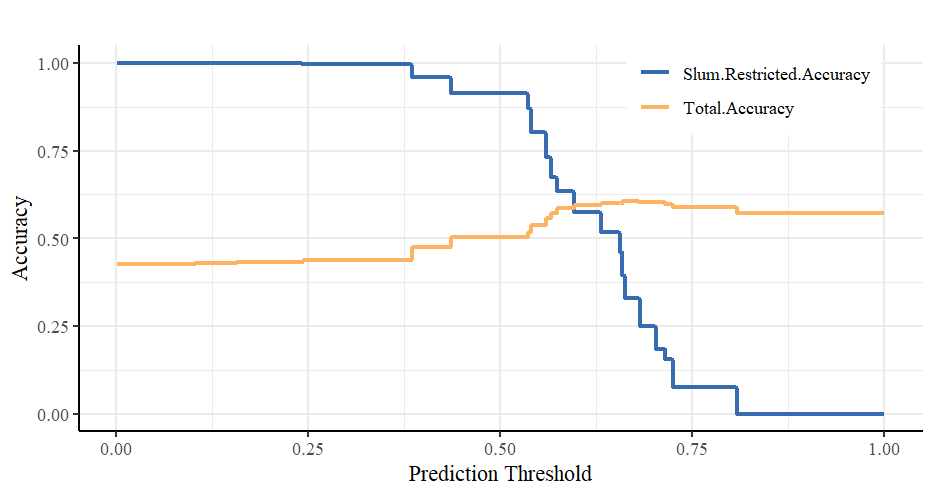
\includegraphics[scale = 0.8]{Graphics/Weighted Slums and Total Dataset Accuracy Tradeoff.png}
    \caption{Weighted Model Slums and Total data set Accuracy Tradeoff}
    \label{fig:weightedModelTradeoff}
\end{figure}



\begin{figure}
    \centering
    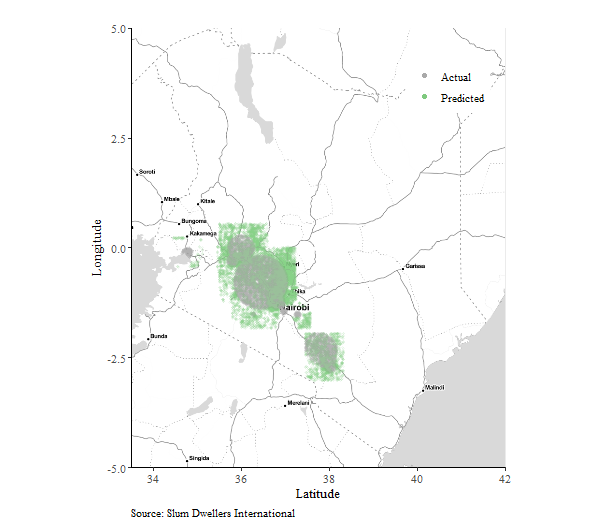
\includegraphics[scale = 0.6]{Graphics/Weighted Predicted Spatial Distribution of Slums in Kenya.png}
    \caption{Weighted Logit Model Predicted Spatial Distribution of Slums in Kenya}
    \label{fig:weightedPredict}
\end{figure}
The error metrics, created at a 0.6 probability prediction threshold level, also seem to fare a bit better for the weighted model. As a whole, the weighted model seems to perform a lot better than the previous two models. There are a lot fewer false positive slum attributions and the overall error metrics also seem to fair a decent proportion better; the qualitative predictive map shows that there are a fewer false positives as well.

\subsubsection{Model 4: Random Forest}

To conclude the predictive modeling portion of the paper we will test a random forest model. This model is a bit different in that it is a blackbox model and so causal interpretability will be much lower than in the previous models; we will not be able to conclude which conditions exactly cause a positive or negative slum observation. Regardless it is a good exercise in identifying if this type of model would have any better predictive power. Similar to the discussion in the previous modeling section, in further applications, data sets may not be as balanced between positive and negative slum observations and decision tree-based classification algorithms tend to be good at addressing these unbalanced data sets.

\begin{figure}
    \centering
    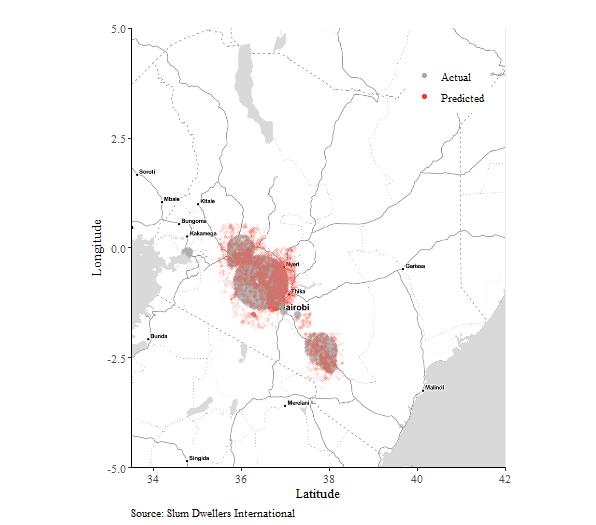
\includegraphics[scale = 0.6]{Graphics/RF Predicted Spatial Distribution of Slums in Kenya.png}
    \caption{Random Forest Model Predicted Spatial Distribution of Slums in Kenya}
    \label{fig:rfPredict}
\end{figure}

\begin{table}[ht]
\centering
\caption{Random Forest variable importance}
\begin{tabular}{ll}
  \hline \hline
  Variable &  Mean Decrease Gini\\ 
  \hline
Nighttime Lights & 5140.58 \\ 
Population Density & 6095.28\\
   \hline
\end{tabular}
\end{table}


In aggregate, the Random Forest model has better error metrics than the first two models but performs worse than the weighted logistic regression. We can see in the map visualization that it doesn't seem to make as many positive slum predictions relatively to the other model and as such its false positive rate is significantly lower than any of the other models. Interestingly enough, the variable importance plots indicate that contrary to the qualitative conclusions of the logit models, population density seems to be more important in making a slum prediction in this Random Forest model.

\begin{table}[ht]
\centering
\caption{Random Forest Model Validation error metrics}
\begin{tabular}{llll}
  \hline \hline
  Error Metric &  Slum Predictions &  Slum Observations  & Error Rate \\ 
  \hline
Total data set & 3399 & 10604 & 0.3564527 \\ 
Positive Slum Observations & 2085 & 4530 & 0.539735099\\
   \hline
\end{tabular}
\end{table}




\subsubsection{Final Comparative Analysis}

Ultimately, each model constructed serves a different purpose contingent on properties of the underlying training data set. Table 13 reports on one yet undiscussed comparative metric: area under curve (AUC) values for the receiver operating characteristic (ROC) curve of each model which provides an aggregate measure of performance across all possible classification thresholds. Note that this is a metric that doesn't capture the best level of error metrics for a model but rather some measure of overall robustness over various classification thresholds. In general, for the AUC values and other error metrics as well we see that there are some definitive differences, and this is especially also made clear in the visual depiction of the predictions that each of the models make. Regardless, the magnitude of the differences in metrics in each of the models speak to the level of robustness of the problem declaration: the ability to be able to map slums based on nighttime light and population density data. Better tuned training data and drawing training data from a larger set of countries may produce a much more accurate model.

\begin{table}[ht]
\centering
\caption{AUC values for ROC curve of each model}
\begin{tabular}{ll}
  \hline \hline
  Model &  AUC\\ 
  \hline
Vanilla Logit & 0.6272 \\ 
Bins Logit & 0.6581\\
Weighted Logit & 0.6272\\
Random Forest & 0.6675385\\
   \hline
\end{tabular}
\end{table}